\documentclass{article}
\usepackage{graphicx}
\usepackage{geometry}
\usepackage{subcaption}
\usepackage{amsmath, amssymb}
\geometry{tmargin=3cm, lmargin=3cm, rmargin=2cm, bmargin=2cm}

\begin{document}
\section{4-component graph}
An experiment with synthetic data generated by a 4-component graph was conducted.
We consider the following model:
\begin{equation}
  \mathbf{L}_{\mathsf{noisy}} = (1 - \kappa) \mathbf{L}_{\mathsf{true}} + \kappa \mathbf{L}_{\mathsf{ER}},
  \label{eq:model}
\end{equation}
where $\mathbf{L}_{\mathsf{true}}$ represents the Laplacian matrix of a $K$-component graph (for this example, $K = 4$)
denoted as $\mathcal{G}^{(p_1, p_2)}_K$,
in which $p_1$ and $p_2$ represent the probabilities of node connections across components and within components, respectively;
$\mathbf{L}_{\mathsf{ER}}$ represents the Laplacian of an Erdos-Renyi graph $\mathcal{G}^{(p)}_{\mathsf{ER}}$, in which $p$
is the probability of a node connecting to any other node; and $\kappa \in (0, 1)$ controls how much noise is added into
$\mathbf{L}_{\mathsf{true}}$ by the Erdos-Renyi model. Additionally, the weighted edges of both $\mathcal{G}^{(p_1, p_2)}_K$
and $\mathcal{G}^{(p)}_{\mathsf{ER}}$ were drawn from $\textsf{Uniform}(0, 1)$. Finally, we set $p_1 = 0$, $p_2 = 1$,
$p = 0.35$, and $\kappa = 0.2$.

Then, data were sampled in the form of $\mathbf{Y} \thicksim \mathcal{N}(\mathbf{0}, \mathbf{L}_{\mathsf{noisy}}^{\dagger})$,
where $\mathbf{A}^{\dagger}$ denotes the generalized inverse of the matrix $\mathbf{A}$. The total number of nodes $N$
and the number of drawn samples $T$ were set to $N = 64$ (16 nodes per component) and $T / N = 30$.

Figure~\ref{fig:4-comp} illustrates the ground truth model, its noisy version, and the model learned by our spectral
topology algorithm with $\beta = 10$. We compute the performance of the learning process by means of the relative error
($\textsf{RE}$) and the F-score ($\textsf{FS}$). For this example, our algorithm achives $(\mathsf{RE}, \mathsf{FS}) = (0.131, 0.993)$
which means almost perfect clustering accuracy even in a noisy model that heavily supress the ground truth weights when $\kappa$ is much
larger than zero.

\begin{figure}[!htb]
    \centering
    \begin{subfigure}[b]{0.3\textwidth}
        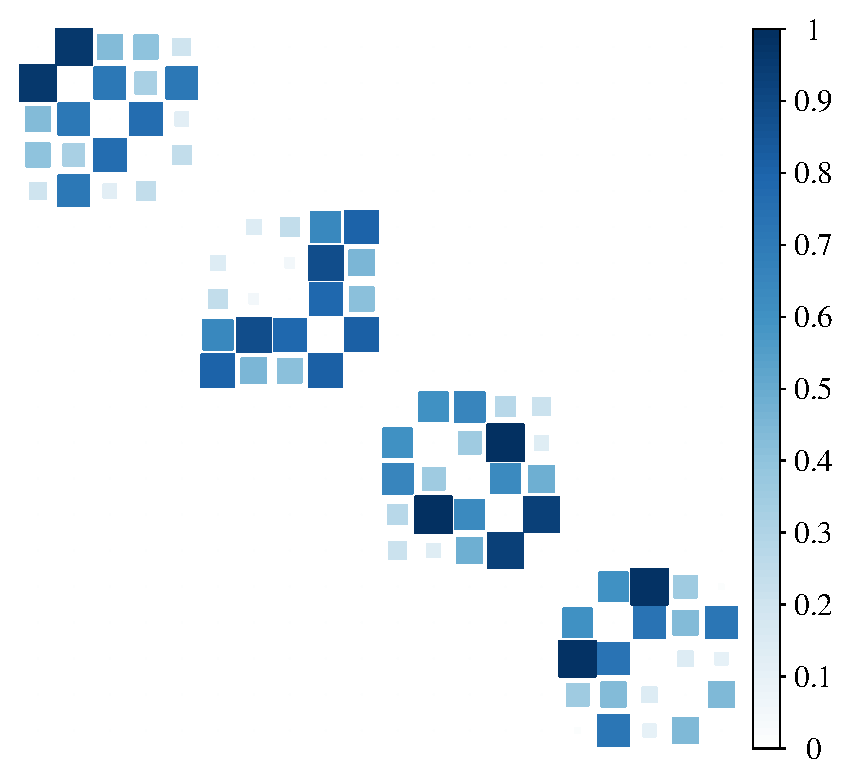
\includegraphics[width=\textwidth]{true_mat.eps}
        \caption{Ground Truth Laplacian matrix}
    \end{subfigure}
    ~ %add desired spacing between images, e. g. ~, \quad, \qquad, \hfill etc.
      %(or a blank line to force the subfigure onto a new line)
    \begin{subfigure}[b]{0.3\textwidth}
        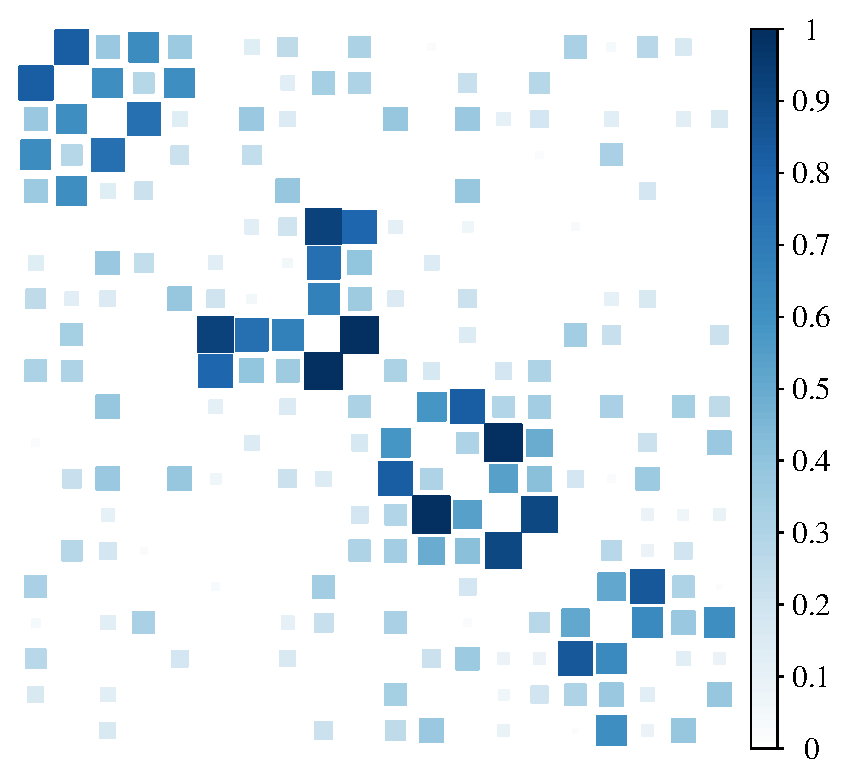
\includegraphics[width=\textwidth]{noisy_mat.eps}
        \caption{Noisy Laplacian matrix}
    \end{subfigure}
    ~ %add desired spacing between images, e. g. ~, \quad, \qquad, \hfill etc.
    %(or a blank line to force the subfigure onto a new line)
    \begin{subfigure}[b]{0.3\textwidth}
        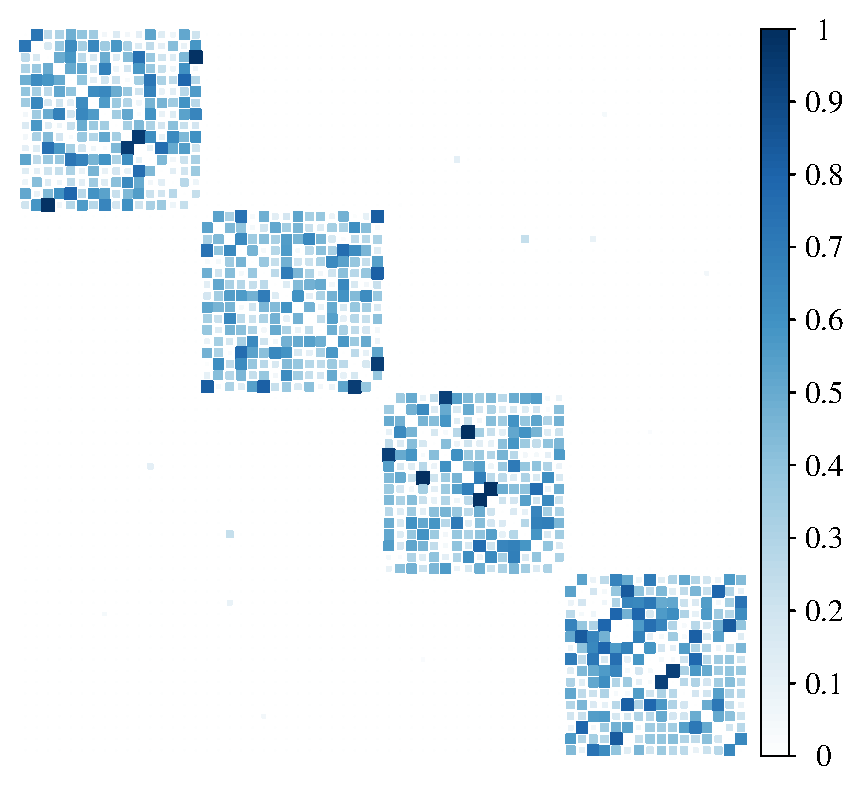
\includegraphics[width=\textwidth]{est_mat.eps}
        \caption{Learned Laplacian matrix}
    \end{subfigure}
        \\
    \begin{subfigure}[b]{0.3\textwidth}
        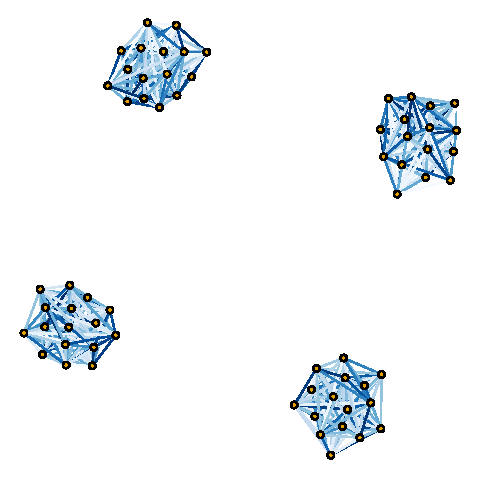
\includegraphics[width=\textwidth]{true_graph.eps}
        \caption{Ground Truth graph}
    \end{subfigure}
    ~ %add desired spacing between images, e. g. ~, \quad, \qquad, \hfill etc.
      %(or a blank line to force the subfigure onto a new line)
    \begin{subfigure}[b]{0.3\textwidth}
        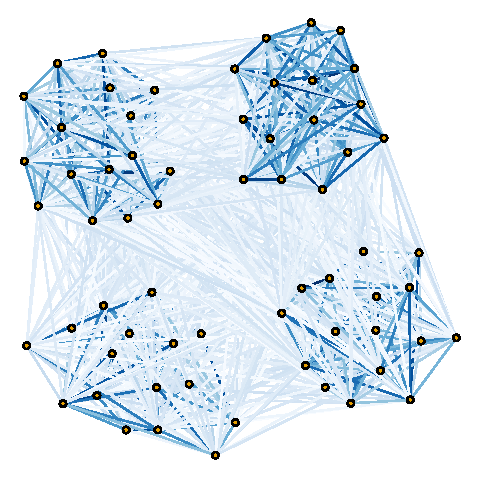
\includegraphics[width=\textwidth]{noisy_graph.eps}
        \caption{Noisy graph}
    \end{subfigure}
    ~ %add desired spacing between images, e. g. ~, \quad, \qquad, \hfill etc.
    %(or a blank line to force the subfigure onto a new line)
    \begin{subfigure}[b]{0.3\textwidth}
        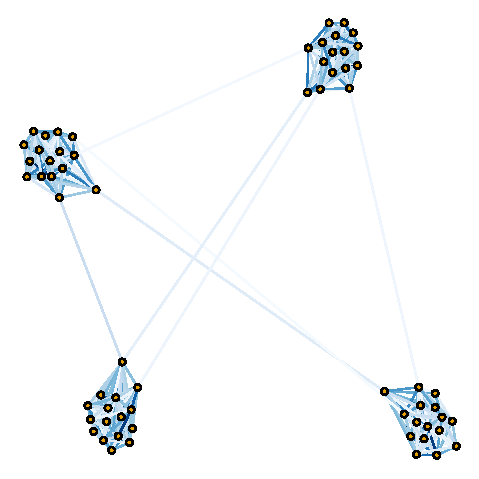
\includegraphics[width=\textwidth]{est_graph.eps}
            \caption{Learned graph}
    \end{subfigure}
        \caption{An example of estimating a 4-component graph. (a) the ground truth graph Laplacian matrix ($\mathbf{L}_{\mathsf{true}}$),
                 (b) $\mathbf{L}_{\mathsf{true}}$ after being corrupted by noise, (c) the learned graph Laplacian with a performance of
                 $(\mathsf{RE}, \mathsf{FS}) = (0.131, 0.993)$..
                 The panels (d), (e), and (f) correspond to the graphs represented by the Laplacian matrices in
                 (a), (b), and (c), respectively.}\label{fig:4-comp-graph}
        \label{fig:4-comp}
\end{figure}

\end{document}
